\section{Ejercicios}

\begin{problem}
Encontrar el lenguaje definido por la gramática:
\begin{itemize}
\item $S \rightarrow abB$
\item $A \rightarrow aaBb$
\item $B \rightarrow bbAa$
\item $A \rightarrow \lambda$
\end{itemize}
\solution
Mediante el elegante método de \textbf{La cuenta de la vieja} llegamos a:

 L(G) = $ab(bbaa)^nbba(ba)^n$
\end{problem}

\begin{problem}
Dado el lenguaje $\Sigma = \lbrace a,b \rbrace$ queremos encontrar las gramáticas, las expresiones regulares y los autómatas finitos deterministas que representen:
\begin{enumerate}
\item Cadenas con exactamente una 'a'
\item Cadenas con al menos una 'a'
\item Cadenas con, como mucho, 3 'a's
\end{enumerate}
\solution

\begin{enumerate}
% Cadenas con sólo una a
\item 
La expresión regular sería: $b^*a b^*$

La gramática que lo representa:

\begin{itemize}
\item $S \rightarrow BaB$
\item $B \rightarrow Bb$
\item $B \rightarrow \lambda$
\end{itemize}

El autómata sería:
\begin{center}
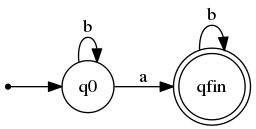
\includegraphics[scale=0.75]{tex/automata1.png}
\end{center}

% Cadenas con al menos una a
\item 
La expresión regular sería: $(a+b)^* a (a+b)^* $

La gramática que lo representa es:
\begin{itemize}
\item $S \rightarrow XaX$
\item $X \rightarrow XZ | \lambda$
\item $Z \rightarrow a | b$
\end{itemize}

El autómata sería:
\begin{center}
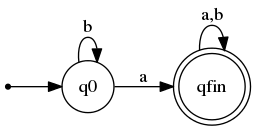
\includegraphics[scale=0.75]{tex/automata2.png}
\end{center}

% Cadenas con como mucho 3 aes
\item 
La expresión regular sería: $b^* (\lambda (a+b) + (a+b)^2 + (a+b)^3) b^*$

Otra expresión podría ser: $b^*(a+b+\lambda)b^*(a+b+\lambda)b^*(a+b+\lambda) b^*$

La gramática que lo representa es:
\begin{itemize}
\item
\item
\end{itemize}

El autómata sería:
\begin{center}
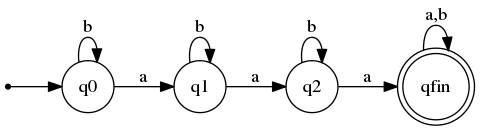
\includegraphics[scale=0.75]{tex/automata3.png}
\end{center}

\end{enumerate}
\end{problem}

\begin{problem}
Dada la siguiente gramática:
\begin{itemize}
\item $S \rightarrow aA$
\item $A \rightarrow bS$
\item $S \rightarrow \lambda$
\end{itemize}
 Encontrar el lenguaje que representa
 \solution
 
 algooo
\end{problem}

\begin{problem}
 Dada la siguiente gramática:
\begin{itemize}
\item $S \rightarrow Aa$
\item $A \rightarrow B$
\item $B \rightarrow Aa$
\end{itemize}
 Encontrar el lenguaje que representa
\solution
algoo

\end{problem}